\chapter{Calibration du modèle} 

\lettrine{O}{n} détaille dans ce chapitre la méthodologie utilisée pour calibrer les paramètres libres du modèle.
On s'intéressera notamment à définir une fonction de coût, pour évaluer la qualité de la calibration.
Dans cette optique, on essayera de calibrer les paramètres en utilisant uniquement les dynamiques du verger n\textdegree1 ; le deuxième servira à la validation.

% Il peut être utile de donner la liste des paramètres à calibrer :
% \begin{itemize}
%  \item $\gamma$, le paramètre relatif à l'arrivée des femelles exogènes ;
%  \item $p_{\text{m}}$, le paramètre relatif à la migration des femelles endogènes entre les sous-parcelles ;
%  \item $\mu^{1}_{\text{ER}}$ et $\mu^{2}_{\text{ER}}$, les probabilité de réussir à entrer et à sortir du sol pour les cécidomyies pour la modalité «enherbement ras». Pour simplifier,
%  on pose $\mu^{1}_{\text{ER}} = \mu^{2}_{\text{ER}}$;
%  \item $\mu^{1}_{\text{EH}}$ et $\mu^{2}_{\text{EH}}$, les probabilité de réussir à entrer et à sortir du sol pour les cécidomyies pour la modalité «enherbement haut». Ici aussi,
%  on pose $\mu^{1}_{\text{EH}} = \mu^{2}_{\text{EH}}$;
%  \item $k$, le paramètre relatif à la disponibilité en ressources pour les inflorescences ;
%  \item \texttt{stock}, le nombre de larves entrées en diapause les années précédentes qui décident de sortir l'année considérée ;
%  \item $E_0\mu_{\ell}$, le nombre d'œufs pondus par une femelle qui survivent, se transforment en larves puis s'éjectent de l'inflorescences. 
% \end{itemize}


\section{Fonction de coût}

Une étape importante pour la calibration du modèle est de définir une fonction de coût qui permet de mesurer la qualité de nos estimations.
Pour ce faire, on utilisera une fonction permettant de comparer le nombre de larves estimées avec le nombre de larves observées.

Il faut cependant noter qu'il n'y a que 20 relevés effectifs, et qu'ils ne furent pas fait à intervalles très réguliers.
Si l'on appliquait notre fonction de coût à chacun des jours de la période considérée, on attribuerait plus d'importance aux relevés qui ont eu un écart relativement important avec le relevé précédent.
Pour pallier ce problème, on comparera uniquement la moyenne des estimations correspondant à un relevé avec l'observation correspondante.
Notre propos est illustré sur la figure~\ref{fig:calib}.
% La comparaison se fera grâce à la fonction NRMSE (Normalized Root Mean Square Error).

\begin{figure}[ht]
\centering
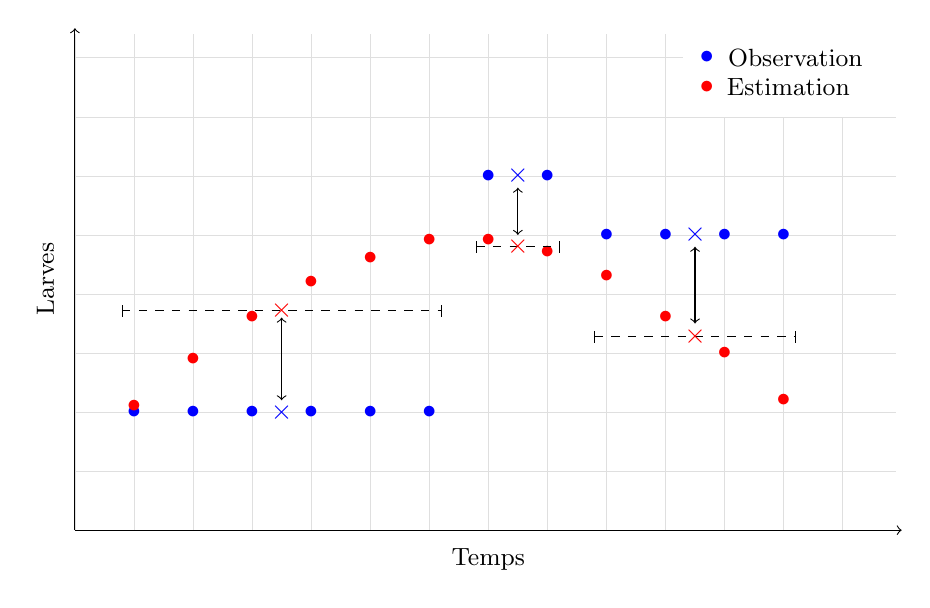
\begin{tikzpicture}[scale = 0.75]
 \draw [very thin, lightgray, opacity = 0.5] (0,0) grid (13.9, 8.4);
 \draw [->] (0, 0) -- (0, 8.5);
 \draw [->] (0, 0) -- (14, 0);
 \draw (1, 2) node{\textcolor{blue}{$\bullet$}};
 \draw (2, 2) node{\textcolor{blue}{$\bullet$}};
 \draw (3, 2) node{\textcolor{blue}{$\bullet$}};
 \draw (4, 2) node{\textcolor{blue}{$\bullet$}};
 \draw (5, 2) node{\textcolor{blue}{$\bullet$}};
 \draw (6, 2) node{\textcolor{blue}{$\bullet$}};
 \draw (7, 6) node{\textcolor{blue}{$\bullet$}};
 \draw (8, 6) node{\textcolor{blue}{$\bullet$}};
 \draw (9 , 5) node{\textcolor{blue}{$\bullet$}};
 \draw (10, 5) node{\textcolor{blue}{$\bullet$}};
 \draw (11, 5) node{\textcolor{blue}{$\bullet$}};
 \draw (12, 5) node{\textcolor{blue}{$\bullet$}};
 \draw (1, 2.1) node{\textcolor{red}{$\bullet$}};
 \draw (2, 2.9) node{\textcolor{red}{$\bullet$}};
 \draw (3, 3.6) node{\textcolor{red}{$\bullet$}};
 \draw (4, 4.2) node{\textcolor{red}{$\bullet$}};
 \draw (5, 4.6) node{\textcolor{red}{$\bullet$}};
 \draw (6, 4.9) node{\textcolor{red}{$\bullet$}};
 \draw (7, 4.9) node{\textcolor{red}{$\bullet$}};
 \draw (8, 4.7) node{\textcolor{red}{$\bullet$}};
 \draw (9, 4.3) node{\textcolor{red}{$\bullet$}};
 \draw (10, 3.6) node{\textcolor{red}{$\bullet$}};
 \draw (11, 3) node{\textcolor{red}{$\bullet$}};
 \draw (12, 2.2) node{\textcolor{red}{$\bullet$}};
 \draw [dashed] (0.8, 3.716) -- (6.2, 3.716) ;
 \draw [dashed] (6.8, 4.8) -- (8.2, 4.8) ;
 \draw [dashed] (8.8, 3.275) -- (12.2, 3.275) ;
 \draw (0.8, 3.616) -- (0.8, 3.816);
 \draw (6.2, 3.616) -- (6.2, 3.816);
 \draw (6.8, 4.7) -- (6.8, 4.9);
 \draw (8.2, 4.7) -- (8.2, 4.9);
 \draw (8.8, 3.175) -- (8.8, 3.375);
 \draw (12.2, 3.175) -- (12.2, 3.375);
 \draw (3.5, 3.716) node{\textcolor{red}{$\times$}};
 \draw (7.5, 4.8) node{\textcolor{red}{$\times$}}; 
 \draw (10.5, 3.275) node{\textcolor{red}{$\times$}};
 \draw (3.5, 2) node{\textcolor{blue}{$\times$}};
 \draw (7.5, 6) node{\textcolor{blue}{$\times$}}; 
 \draw (10.5, 5) node{\textcolor{blue}{$\times$}}; 
 \draw [<->] (3.5, 2.2) -- (3.5, 3.6);                  
 \draw [<->] (7.5, 5.8) -- (7.5, 5);
 \draw [<->] (10.5, 4.8) -- (10.5, 3.5);
 \draw [fill=white,white] (10.3, 7.01) rectangle (13.9, 8.4);
 \draw (12.2, 8) node {{\small Observation}};
 \draw (12.08, 7.5) node {{\small Estimation}};
 \draw (10.7, 8) node{\textcolor{blue}{$\bullet$}};
 \draw (10.7, 7.5) node{\textcolor{red}{$\bullet$}};
 \draw (6, 0.135) node[rotate = 180] {\textcolor{ForestGreen}{$\intercal$}};
 \draw (8, 0.135) node[rotate = 180] {\textcolor{ForestGreen}{$\intercal$}};
 \draw (12, 0.135) node[rotate = 180] {\textcolor{ForestGreen}{$\intercal$}};
 \draw (7, -0.5) node{\small \text{Temps}};
 \draw  (-0.5, 4.25) node{\rotatebox{90}{\small Larves}};
\end{tikzpicture}
\caption{Schéma illustrant le fonctionnement de la fonction objectif. À chaque relevé effectif (marqueurs verts), on fait correspondre la période correspondant à ce relevé (segments en pointillés).
Et pour chacune de ces périodes, on calcule la moyenne des valeurs estimées (les croix rouges). On compare ensuite les moyennes ainsi calculées avec les valeurs observées associées (les croix bleues).}
\label{fig:calib}
\end{figure}

Pour définir la fonction de coût, on pose :
\begin{itemize}
 \item $m$, le nombre de jours entre la première observation et la dernière ;
 \item $n$, le nombre de relevés effectif;
 \item $t$, le nombre de jours passés depuis la première observation ;
 \item $t^j$, le nombre de jours entre la première observation et le $j^{\text{ème}}$ relevé.
\end{itemize}
(On a donc $t^1 = 0$ et $t^n = m$.)

Si l'on note les observations $y$ et les estimations $\hat y$, notre fonction de coût peut s'écrire
$$
f(y, \hat y) = \frac{\sqrt{\frac{1}{n-1}\sum_{j=2}^n\left( y^*_j - \hat y^*_j \right)^2}}{\max_j(y^*_j) - \min_j(y^*_j)},
$$
où 
$$y^*_j =  y_{t^j}, \qquad \text{ et } \qquad \hat y^*_j = \frac{1}{t^j - t^{j-1}}\sum_{k=t^{j-1}}^{t^j} \hat y_k.$$
Concrètement $\hat y^*_j$ donne la moyenne des estimations correspondant à un relevé et $y^*_j$ donne la valeur observée associée.
Appliquer la fonction à $n-1$ valeurs (correspondant aux relevés sur le terrain) plutôt qu'à chacun des $m$ jours (correspondant à l'étendue des relevés) de ne pas attribuer plus d'importance aux relevés qui ont eu un écart relativement important avec le relevé précédent.




Par la suite, l'objectif sera de minimiser cette fonction pour chacune des trois sous-parcelles.

\section{Analyse de sensibilité}

Avant de calibrer le modèle, il est pertinent d'effectuer une analyse de sensibilité.
L'analyse de sensibilité est définie par \citet{saltelli2004} comme
\begin{quote}
 «l'étude de comment l'incertitude de la sortie d'un modèle --- qu'elle soit numérique ou non --- peut être répartie entre les différentes sources d'incertitudes présentes dans les entrées du modèle.»\footnote{«The study of how uncertainty in the output of a model (numerical or otherwise) can be apportioned to different sources of uncertainty in the model input.»}
\end{quote}
Autrement dit, on cherche à connaître les paramètres les plus influants sur la sortie du modèle.
La calibration comportant toujours une part d'arbitraire, cette analyse permet de prendre du recul sur les choix de paramètres, relativement à leur impact sur les sorties du modèle.
% En particulier lorsque certains paramètres ne sont qu'approximatifs vis à vis de la réalité qu'ils ont vocation à décrire, mais fortement significatifs pour la sortie du modèle.

Il existe deux grandes catégories d'analyses de sensibilité, celles qui ont une approche globale et celles qui ont une approche locale (parfois appelées \emph{one-at-the-time}).
L'approche locale consiste à étudier la sensibilité des paramètres les uns après les autres, les uns indépendamment des autres.
Cette approche est valable si et seulement si le modèle est linéaire par rapport à chacune de ses entrées $x_i$ et qu'il n'y a aucune interaction entre les différentes entrées du modèle \citep{saltelli2019so}.
Dès lors qu'il y a la moindre incertitude sur la linéarité du modèle ou sur la non-interaction entre les paramètres, il faut privilégier une approche globale.
Notre modèle n'est pas linéaire et il n'y a dans notre cas aucune raison de supposer la non-interaction entre nos paramètres, bien au contraire.
On utilisera donc une approche globale.

Bien qu'il existe plusieurs méthodes ayant une approche globale, elles ont toutes en commun de fonctionner dans un cadre non-linéaire et de prendre en compte les différentes interactions entre les différents paramètres.
Parmi les méthodes les plus connues et les plus utilisées, on peut en citer qui fonctionnent par décomposition de la variance comme Sobol ou FAST (Fourier Amplitude Sensitivity Test) ou d'autres qui fonctionnent en effectuant des perturbations élémentaires des entrées du modèle comme la méthode Morris.
Notre modèle possède moins de 20 paramètres et s'exécute en moins d'une minute, nous utiliserons alors la méthode Sobol conformément aux recommendations de \citet[chap. 6]{saltelli}.

Le fonctionnement de cette méthode est relativement intuitif.
On considère que la sortie de notre modèle $Y$ peut s'exprimer comme une fonction des entrées de notre modèle $X,$ c'est-à-dire $Y = f(X)$.
Comme $X = \left( X_1, \ldots, X_p \right)$ peut prendre un nombre important de valeurs possibles, il en résulte qu'il y a \emph{a priori} un nombre important de résultats possibles pour $Y.$
% L'objectif est alors de décomposer ces résultats possibles --- cette variance qu'admet $Y$ --- en fonction de chaque entrée du modèle $X_i$.
L'objectif est alors de déterminer quelles entrées du modèle $X_i$ induisent le plus de changements dans ces résultats possibles --- dans cette variance qu'admet $Y.$
À cette fin, on utilise les indices principaux de Sobol définis par
\[
S_i = \frac{\textbf{Var}\!\left( \mathbf{E}\!\left[Y|X_i\right] \right)}{\textbf{Var}\!\left( Y \right)}.
\]
% L'indice $S_i$ permet de voir l'effet du seul paramètre $X_i$ sur la variance de $Y$ relativement aux autres.
Ici, $\textbf{Var}\!\left( \mathbf{E}\left[Y|X_i\right] \right)$ permet de voir l'effet du seul paramètre $X_i$ sur la variance de $Y.$
Diviser par la variance totale de $Y$ permet de le faire relativement aux autres paramètres.
Cet indice ne prend cependant pas en compte les interactions entre $X_i$ et les autres entrées du modèle. 
Il faut pour ça utiliser les indices totaux de Sobol définis par
\[
S^T_i = 1 - \frac{\textbf{Var}\!\left( \mathbf{E}\!\left[Y|X_{\sim i}\right] \right)}{\textbf{Var}\!\left( Y \right)},
\]
où $X_{\sim i} = \left(X_1, \ldots, X_{i-1}, X_{i+1}, \ldots, X_p \right)$.
L'indice $S^T_i$ ainsi défini permet lui de prendre en compte l'impact du paramètre $X_i$ et de ses interactions sur la variance de $Y$.
À noter que l'interaction entre $X_i$ et $X_j$ est à la fois prise en compte par $S^T_i$ et $S^T_j$.
C'est pour cette raison qu'il est souvent pertinent d'interpréter les indices principaux et les indices totaux conjointement.

Une fois que l'on connaît la sensibilité du modèle aux différents paramètres, on peut alors passer à la calibration desdits paramètres.


\section{Algorithme d'optimisation}

L'objectif de l'optimisation est de trouver les jeux de paramètres qui minimisent notre fonction de coût, ceux qui permettent d'ajuster au mieux les dynamiques de larves simulées aux dynamiques observées.
Pour ce faire, un algorithme d'optimisation est nécessaire.


On peut déjà noter que nous avons sept paramètres à calibrer, et qu'ils évoluent tous dans des intervalles (que l'on définira plus tard).
Il apparaît évident qu'un test de exhaustif de toutes les valeurs de paramètres est trop coûteux.
Une approche peut être d'utiliser un algorithme basé sur une méthode MCMC comme l'algorithme du recuit simulé.
Nous avons cependant trois dynamiques à ajuster (une pour chaque sous-parcelle), il faudrait alors minimiser la somme (ou la moyenne) des trois fonctions objectifs.

Une alternative est d'utiliser un algorithme d'optimisation multicritères.
Ces algorithmes ont l'avantage de pouvoir optimiser simultanément des objectifs qui ne sont pas toujours comparables --- à des échelles différentes, par exemple.
Un des plus connus est sans conteste l'algorithme génétique NSGA-II (Nondominated Sorting Genetic Algorithm II) \citep{deb}.
C'est celui que nous avons testé.

C'est un algorithme qui ne renvoie pas une unique solution mais un ensemble de solutions. 
Cet ensemble de solutions converge vers un sous-ensemble du front de Pareto.
Le front de Pareto désigne l'ensemble des solutions non-dominées pour un problème donné.
Dans $P \subset \mathbf{R}^{p}$ ($p$ > 1), une solution $x^* = \left( x_1, \ldots, x_p \right) \in  P$ est dite non-dominée lorsque
\[
\left\{ x \in P\ |\ \forall\ i \in \{1, \ldots, p\},\ x_i \succcurlyeq x_i^* \text{ et } \exists\ i \text{ tel que } x_i \succ x_i^* \right\} = \emptyset,
\]
où $\succcurlyeq$ et $\succ$ veulent respectivement dire «est préféré à» et «est strictement préféré à». 
Dans notre cas, vu que l'on veut minimiser notre fonction de coût, $x^* \succcurlyeq x$ se traduira par $f(x^*) \leq f(x)$ et $x^* \succ x$ se traduira par $ f(x^*) < f(x)$, où la fonction $f$ représente la composée de notre modèle suivi de notre fonction de coût.
En d'autres termes, $x$ est non-dominée signifie qu'il n'existe pas de solution $y$ qui soit strictement meilleure sur un des critères et au moins aussi bonne sur tous les autres critères.

Le front de Pareto étant un sous-ensemble de $\mathbf{R}^{p}$, il n'est (\emph{a priori}) pas dénombrable.
De ce fait, NSGA-II ne peut pas renvoyer le front tout entier mais seulement un sous-ensemble.
C'est un algorithme itératif, et les itérations seront appelées ici \emph{générations}.
C'est un algorithme convergent, plus il y a de générations, plus les solutions proposées sont proches du front de Pareto.
En pratique, il ne renvoie donc pas un sous-ensemble du front de Pareto mais un ensemble de solutions se rapprochant d'un sous-ensemble du front de Pareto.

À la génération $t$, l'algorithme effectue plusieurs opérations.
\begin{enumerate}
 \item On possède un ensemble de solutions potentielles que l'on nommera \emph{population}.
 La taille de la population $N$ est fixée arbitrairement.
 \item À chaque solution de cette population $P_t$, on attribue une solution fille (on verra la suite comment). 
\end{enumerate}

 Avec la population $P_t$ et les solutions filles associées $O_t$ (\emph{offspring} en anglais), cela forme un ensemble de solutions potentielles $S_t$ de taille $2N$. 
 On va alors sélectionner parmi ces solutions les $N$ solutions les moins dominées possibles.
\begin{enumerate}[resume]
 \item Pour ce faire, pour chaque solution potentielle $s\in S_t$ :
 \begin{itemize}
  \item on établit l'ensemble $D_s$ d'élément de $S_t$ qui sont dominées par $s$. On note $n_s$ son cardinal ;
  \item on établit l'ensemble $E_s$ des autres solutions de $S_t$ qui sont dominées par la solution $s$.
 \end{itemize}
 \item On répartit alors nos solutions en plusieurs groupes, en plusieurs \emph{fronts}.
 Vont ainsi dans le premier front $F^1$ les solutions $s$ qui vérifient $n_s = 0$, qui ne sont donc pas dominées par d'autres solutions de $S_t$. 
 Dans le deuxième front $F^2$ se trouvent les solutions qui sont dominées uniquement par les solutions présentes dans $F^1$.
 (Autrement dit, les solutions qui se trouvent dans et uniquement dans $\bigcup_{s\in F_1} E_s$.)
 On continue de la même manière pour $F^3$ qui contient les solutions uniquement dominées par celles de $F^2$ (et \emph{a fortiori} par $F^1$), $F^4$... jusqu'à ce que toutes les solutions de $S_t$ soient assignées à un front.
 \item On choisira alors de garder en priorité les solutions de $F^1$ puis de $F^2$ et ainsi de suite jusqu'à en obtenir $N$. 
 Il faut noter qu'il existe probablement un front $F^k$ où toutes les solutions ne pourront être garder pour ne pas dépasser la limite imposée de $N$ solutions.
 Plutôt que de choisir aléatoirement le nombre nécessaires de solutions dans $F^k$, seront sélectionnées les solutions qui maximisent une certaine distance --- the \emph{crowding distance} --- avec les autres solutions.
 (On n'entrera pas dans le détail ici.)
 C'est fait pour assurer une certaine diversité entre les différentes solutions.
 Les $N$ solutions ainsi sélectionnées constitueront $P_{t+1}$, la population initiale de la génération suivante $t+1$.
\end{enumerate}

Un élément important pour assurer une convergence vers le front de Pareto est le choix des solutions filles $O_t$ effectué à chaque génération.
Bon nombres d'algorithmes génétiques (dont NSGA-II) utilisent la \emph{sélection}, le \emph{crossover} et la \emph{mutation} pour générer une solution fille.
La sélection consiste à choisir certaines solutions mères qui seront les mieux à même de produire une bonne solution fille.
Dans notre cas, les solutions du front $F^1$ seront choisies avec une plus grande probabilité que les autres
Le crossover consiste à créer une solution fille en mélangeant des coordonnées de deux solutions mères sélectionnées.
La mutation effectue un changement aléatoire sur une des coordonnées, ce qui favorise la diversité des solutions.

% Ces étapes simplifiées sont :
% \begin{enumerate}
%  \item On sélectionne deux solutions $s_1$ et $s_2$ dans $P_t$.
%  \item On construit une solution fille $f_1$ en prenant la moitié des coordonnées de $s_1$ et l'autre moitié de $s_2$. 
%  On construit $f_2$ en prenant les moitiés de $s_1$ et $s_2$ inutilisées dans la construction de $f_1$.
%  \item Sur chacune des solutions filles, une coordonnée choisie aléatoirement est remplacée par une valeur aléatoire choisie dans un intervalle centré sur la valeur initiale.
%  \item On réitère ces étapes jusqu'à avoir $N$ solutions filles.
% \end{enumerate}


Et c'est ainsi qu'après un nombre suffisant d'itérations, et pour une taille de population suffisamment grande, l'algorithme NSGA-II renvoie un ensemble de points suffisamment proche du front de Pareto et qui en retranscrit sa diversité.


Dans notre cas, cela signifie que l'on possède différents jeux de paramètres et les valeurs de la fonction de coût pour les trois sous-blocs qu'ils produisent.
Et qu'il ne reste plus qu'à faire un choix.



\section{Exploration de l'ensemble des solutions}


Choisir une solution n'est cependant pas trivial.
En effet, parmi les solutions possibles, aucune n'est objectivement meilleure que les autres.
Il en découle que le choix sera forcément arbitraire.

Plusieurs approches sont possibles.
On peut par exemple choisir au hasard un nombre restreint de jeux de paramètres possibles, les tester puis sélectionner celui qui semble le plus pertinent.
On peut aussi sélectionner le jeu de paramètre qui minimise une norme sur nos trois critères, en estimant qu'il représente un bon compromis entre les différents critères.

On préférera une autre approche. 
Puisque NSGA-II essaye de renvoyer des solutions couvrant au maximum le front de Pareto, cela implique que certains de nos jeux de paramètres auront des valeurs proches.
Et qu'elles renverront donc des dynamiques similaires.
Il peut être donc pertinent d'effectuer une classification non-supervisée de nos solutions afin de recenser les différentes solutions-types.
Pour ce faire, on peut effectuer une classification ascendante hiérarchique (CAH).

Le principe est le suivant.
On traduit nos jeux de paramètres centrés -- réduits dans un espace métrique. On choisira $\mathbf{R}^p$ muni de la distance euclidienne.
% Plus deux solutions seront proches du point de vue de la distance euclidienne, plus elles seront semblables et appartiendront \emph{a priori} à la même classe de solutions.
On cherche à rassembler les différents jeux de paramètres en différentes classes.
Les classes se doivent de contenir des individus aussi proches que possible (\emph{i.e.} la distance entre un individu de la classe et l'individu moyen de la classe doit être petite), et être aussi différentes des autres classes que possible (\emph{i.e.} la distance entre l'individu moyen de la classe et l'individu moyen de la classe la plus proche doit être grande).
D'un point de vue formel, cela peut s'exprimer par la décomposition de l'inertie totale en inertie externe des classes et en inertie interne des classes.
Cette décomposition est donnée par
\[
\underbrace{\frac{1}{n}\sum_{i=1}^{n} \lVert x_i \rVert^2}_{\text{inertie totale}} = \underbrace{\sum_{k=1}^{K}w^k\lVert \overline{x}^{k} \rVert^2}_{\text{inertie externe}} +
\underbrace{\sum_{k=1}^{K} \sum_{x_i\in C_k} \frac{1}{n} \lVert x_i - \overline{x}^k \rVert^2}_{\text{inertie interne}},
\]
où $K$ représente le nombre de classes, $w^k$ le poids de la classe $C_k$ et $\overline{x}^{k}$ l'individu moyen de la classe $C_k$.
L'objectif est alors de trouver les classes $C_k$ qui minimisent l'inertie interne et qui maximise l'inertie externe.
Cependant, les classes $C_k$ dépendent du nombre de classes $K$, et ce nombre est choisi par l'utilisateur de la méthode.
Il est évident que plus il y a de classes, plus l'inertie intra-classe sera faible ; néanmoins la classification a pour but de rassembler les individus, avoir maintes classes n'est alors pas très pertinent.
On reviendra sur le choix de $K$ plus tard.

Initialement, la CAH commence avec $n$ classes : chaque individu se trouve dans une classe ne contenant que lui.
Et à chaque étape, on regroupe deux classes similaires jusqu'à n'en avoir plus qu'une unique contenant tous les individus.
Les deux classes qui sont regroupées à chaque étape sont choisies car elles minimisent un \emph{indice d'agrégation}.
Il en existe un certain nombre, nous choisirons comme indice d'agrégation l'indice de Ward.
Il est défini par
\[
\mu\left( C_k, C_{\ell} \right) = \frac{w^kw^{\ell}}{w^k + w^{\ell}}\lVert \overline{x}^k - \overline{x}^{\ell} \rVert^2,
\]
où $w^k$ est le poids de la classe $k$ et $\overline{x}^k$ est l'individu moyen de la classe $k$.
Cet indice a l'avantage d'être exprimable en fonction de l'inertie, et notamment de l'inertie intra-classes que l'on souhaite minimiser \citep{bry}.
% Lorsque l'on a qu'une unique classe, l'inertie intra-classe est égale à l'inertie totale, et lorsque l'on a 

Ainsi, la CAH donne les classes $C_k$ pour tous les nombres de classes possibles, \emph{i.e.} $K = 1,\ldots, n$.
Il ne reste plus qu'à choisir $K$.
Agréger deux classes a un certain coût qui se traduit par une augmentation de l'inertie intra-classes.
Donc \emph{a fortiori}, réduire le nombre de classes est une bonne chose si l'augmentation de l'inertie intra-classes est minime.
En pratique, on choisira un nombre de classes $K^*$ qui minimisera significativement l'inertie intra-classes par rapport à celle obtenue avec $K^* -1$ classes.

Il faut aussi noter que dans notre cas précis, cette classification est faite dans un but exploratoire. 
Il vaudra mieux avoir un nombre de classes délibérément grand, quitte à avoir des classes semblables, afin de ne pas passer à côté d'une catégorie de solutions intéressante.

La pertinence biologique des classes de paramètres trouvées sera finalement validé par des experts.




% Ou alors on essaye d'avoir une vision globale de l'ensemble des solutions.
% Il peut même être pertinent de comprendre voire d'\emph{expliquer} quel jeu de paramètres génère quelle solution.
% Le choix du jeu de paramètre sera alors plus réfléchi, bien que toujours arbitraire.
% 
% Plus précisément, on possède les valeurs de la fonction de coût de nos critères rassemblées dans un tableau $Y$.
% On possède également les jeux de paramètres (nos solutions) responsables de ces valeurs rassemblés dans un tableau $X$.
% Le but serait alors d'explorer $Y,$ pour savoir par exemple si les critères sont antagonistes (\emph{e.g.} améliorer la prédiction sur une sous-parcelle ne détériore-t-elle pas la prédiction de la sous-parcelle voisine ?) ou alors totalement indépendant.
% Mais aussi de pouvoir dire quelles sont les valeurs pour les paramètres $X$ qui minimisent quel critère de $Y$. 
% À cette fin, on peut choisir entre deux méthodes : l'ACP-VI  et la régression PLS2.
% Nous choisirons la régression PLS2 qui, contrairement à l'ACP-VI, est une méthode régularisante \citep{bry}.
% Ce choix nous préserve d'un éventuel problème d'inversibilité de la matrice $X'X$.
% 
% On s'intéresse au fonctionnement de la régression PLS2. 
% On considère que les tableaux $X$ et $Y$ sont centrés-réduits, $X$ est de dimension $n\times p$, $Y$ est de dimension $n\times q$ et que le rang de $X$ est égal à $a$.
% Comme l'explique \citet{tenenhaus}, l'objectif de la régression PLS2 est la «décomposition du tableau $X$ orientée vers l'explication du tableau $Y$».
% Si l'on note $\{t_1,\ldots, t_a\},$ une base orthonormée de $X,$ alors il existe des vecteurs $p_h$ tel que l'on puisse écrire
% \[
% X = \sum_{j = 1}^a t_h p_h'.
% \]
% Le but est de trouver les composantes $t_h$ qui réalisent un compromis entre deux objectifs. 
% Les premières composantes de la base doivent capturer un maximum d'inertie de $X$ en vue d'en réduire la dimension.
% Et aussi permettre de prédire au mieux le tableau $Y.$
% 
% Le choix de la $h^{\text{ème}}$ composante peut se faire comme suit :
% \begin{enumerate}
%  \item On s'intéresse à l'information de $X$ qui n'est pas résumée par les $h-1$ premières composantes. 
%  Elle est donnée par les résidus de $X$ définis par
%  \[
%  X^{h-1}_{\cdot j} = X_{\cdot j} - \sum_{\ell=1}^{h-1} p_{\ell j}t_{\ell},  \quad \text{avec } j = 1,\ldots, p.
%  \]
%  On s'intéresse aussi à l'information de $Y$ qui n'est pas expliquée par les $h-1$ premières composantes de $X$. 
%  Cette information est donnée par les résidus de $Y,$
%  \[
%  Y^{h-1}_{\cdot k} = Y_{\cdot k} - \sum_{\ell=1}^{h-1} c_{\ell k}t_{\ell},  \quad \text{avec } k = 1,\ldots, q.
%  \] 
%  \item On initiale $u_h$ avec la première colonne de $Y^{h-1}$,
%  \[
%  u_h = Y^{h-1}_{\cdot 1}.
%  \]
%  \item On effectue une régression des moindres carrés ordinaires de $X^{h-1}_{\cdot j}$ sur $u_h$ qui passe par l'origine. 
%  La pente de cette droite de régression est déterminée par
%  \[
%  w_{hj} = \frac{X^{h-1'}_{\cdot j} u_h}{u_h'u_h}.
%  \]
%  On pose $w_h = (w_{h1}, \ldots, w_{hp})'$.
%  \item On effectue une régression des moindres carrés ordinaires de $X^{h-1}_{i \cdot} = X_{i\cdot} - \sum_{\ell=1}^{h-1}t_{\ell i}p_{\ell}$ sur $w_h$ qui passe par l'origine. 
%  La pente de cette droite de régression est déterminée par
%  \[
%  t_{hi} = \frac{X^{h-1'}_{i\cdot} w_h}{w_h'w_h}.
%  \]
%  On pose $t_h = (t_{h1}, \ldots, t_{hn})'$.
%  \item On réalise ensuite une régression de $Y^{h-1}_{\cdot k}$ sur $t_h$.
%  La pente de la droite de régression des moindres carrés qui passe par l'origine est donnée par
%  \[
%  c_{hk} = \frac{Y^{h-1'}_{\cdot k} t_k}{t_k't_k}.
%  \]
%  On pose $c_h = (c_{h1}, \ldots, c_{hq})'$.
%  \item On met à jour notre vecteur $u_h$ en effectuant une régression de $Y^{h-1}_{i \cdot} = Y_{i\cdot} - \sum_{\ell=1}^{h-1}t_{\ell i}c_{\ell}$ sur $c_h$.
%  La pente de la droite de régression passant par l'origine nous donne 
%  \[
%  u_{hi} = \frac{Y^{h-1'}_{i \cdot} c_h}{c_h'c_h}.
%  \]
%  On obtient ainsi notre nouveau vecteur $u_h = (u_{h1}, \ldots, u_{hn})'$.
%  \item On réitère les étapes 3 à 6 jusqu'à ce que le vecteur $w_h$ ait convergé.
%  \item Enfin, la pente de la droite de régression des moindres carrés de $X^{h-1}_{\cdot j}$ sur $t_h$ qui passe par l'origine nous donne les coefficients $p_{hj}$.
%  Ils sont définis par
%  \[
%  p_{hj} = \frac{X^{h-1'}_{\cdot j} t_h}{t_h't_h}.
%  \]
%  On en déduit le vecteur $p_h = (p_{h1}, \ldots, p_{hp})'.$
%  \end{enumerate}
% 
% En plus du formalisme, \citet{tenenhaus} nous donne quelques propriétés sur les différents vecteurs :
% \begin{align}
% %  t_h't_{\ell} &= 0  &\text{si $\ell \neq h$,} \\
%  w_h'p_h &= 1,  \\
% %  w_h'X_{\cdot \ell}' &= 0 &\text{pour tout $(h, \ell)$,}\\
%  w_h'p_{\ell} &= 0 &\text{si $\ell \neq h$,}\\
%  w_h'w_{\ell} &= 0 &\text{si $\ell \neq h$,}\\
% %  t_h'X_{\cdot \ell} &= 0 &\text{pour tout $(h, \ell)$,}\\
% %  X^{h} &= X\prod_{j=1}^h\left( I - w_jp_j' \right) &\text{pour $h \geq 1$,}\\
%  t_h &= X'w_h^* &\text{avec $w_h^* = w_h (p_h'w_h)^{-1}$.} \label{txw}
% \end{align}
% Ces propriétés s'avèrent utiles pour exprimer $Y$ en fonction des composantes $t_h$, et donc \emph{a fortiori} en fonction de $X$.
% Admettons que le nombre de composantes retenues soit $H$.
% Par définition des coefficients $c_h$, on peut écrire 
% \[
% Y = t_1c_1' + \cdots + t_Hc_H' + Y^{H},
% \]
% où $Y^{H}$ représente les résidus de $Y$, \emph{i.e.} la part de $Y$ qui n'est pas prédite par les composantes $t_1,\ldots,t_H.$
% Il peut être utile d'alléger l'écriture en posant $T_H = [t_1 | \cdots | t_H]$. 
% On définit $C_H$, $P_H$, $W_H$ et $W_H^*$ de la même manière.
% Ainsi,
% \begin{align*}
%  Y &= T_HC_H' + Y^H\\
%  &= XW_H^*C_H' + Y^H & \text{en utilisant la propriété~\ref{txw},}\\
%  &= XW_H\left( P_H'W_H \right)^{-1}C_H' + Y^H
% \end{align*}
% On en déduit $B = W_H\left( P_H'W_H \right)^{-1}C_H'$ correspondant aux coefficients de la régression PLS2 de $Y$ sur $X$ effectué avec $H$ composantes.
% Ce qui donne
% \begin{align*}
% Y_{\cdot k} &\simeq c_{1k}t_1 + \cdots + c_{Hk}t_H\\
% &\simeq \left( c_{1k}w_{11}^* + \cdots + c_{Hk}w_{H1}^* \right)X_{\cdot 1} + \cdots + \left( c_{1k}w_{1p}^* + \cdots + c_{Hk}w_{Hp}^* \right)X_{\cdot p}\\
% &\simeq b_{k1}X_{\cdot 1} + \cdots + b_{kp}X_{\cdot p}.
% \end{align*}
% Les variables de $X$ étant centrées-réduites, cela signifie que plus le coefficient $b_{kj}$ sera élevé, plus le paramètre $j$ sera déterminant dans la valeur du critère $k$.
% 
% 
% 
% 
% 
% 




